\section{Risoluzione del problema}\label{sec:qiskit}

Per simulare il problema di ottimizzazione del portafoglio, 
abbiamo utilizzato un approccio basato su un modello generativo 
per produrre dati storici. La generazione dei dati è stata 
realizzata tramite una classe fornita da Qiskit, \texttt{RandomDataProvider}, 
che, a partire da parametri come il numero di asset, il 
periodo temporale e un seme per la riproducibilità, ha 
prodotto una tabella di valori rappresentante l'andamento dei 
prezzi degli asset nel tempo (Tabella~\ref{tab:dati-tickers}). 
Inoltre, per rendere più intuitiva la visualizzazione dei dati, 
abbiamo sviluppato uno script che crea un grafico per ciascun asset, 
rappresentando l'andamento temporale dei prezzi (Figura~\ref{fig:graficiAssets}).

\begin{table}[h]
    \centering
    \renewcommand{\arraystretch}{1.5}
    \begin{tabular}{|c|c|c|c|c|}
    \hline
    \textbf{Data} & \textbf{Ticker\_0} & \textbf{Ticker\_1} & \textbf{Ticker\_2} & \textbf{Ticker\_3} \\
    \hline
    2016--01--01 & 80.0573 & 38.8648 & 69.2682 & 76.1653 \\
    \hline
    2016--01--02 & 80.3390 & 38.7966 & 69.5354 & 76.6583 \\
    \hline
    2016--01--03 & 79.4722 & 39.0100 & 70.7954 & 76.0500 \\
    \hline
    \ldots & \ldots & \ldots & \ldots & \ldots \\
    \hline
    \end{tabular}
    \caption{Esempio di dati generati dalla classe \texttt{RandomDataProvider} 
        con un numero di asset uguale a 4 e un periodo temporale che parte dal 2016--01--01.}
    \label{tab:dati-tickers}
\end{table}

Successivamente, sono stati calcolati i rendimenti medi per ciascun asset 
(Formula~\ref{eqn:matriceRendimentiAttesi}) e la matrice di covarianza 
(Formula~\ref{eqn:matriceCovarianza}) utilizzando i metodi offerti dalla 
classe \texttt{RandomDataProvider}. Questi due elementi rappresentano una 
componente fondamentale per l'ottimizzazione del portafoglio, in quanto i 
rendimenti medi forniscono una misura dell'aspettativa di guadagno, mentre 
la matrice di covarianza descrive la relazione tra le variazioni dei prezzi 
dei diversi asset.

I calcoli sono stati effettuati mediante i seguenti metodi:
\begin{lstlisting}[language=python, caption={Calcolo dei rendimenti attesi e della matrice di covarianza.}]
 mu = data_provider.get_period_return_mean_vector()
 sigma = data_provider.get_period_return_covariance_matrix()
\end{lstlisting}

Per favorire una migliore comprensione e visualizzazione della matrice di 
covarianza, ne è stato generato un grafico (Figura~\ref{fig:matriceCovarianza}): 
questo consente di evidenziare visivamente le correlazioni tra i diversi asset.

\begin{figure}[h!]
    \centering
    \begin{subfigure}{0.52\textwidth}
        \centering
        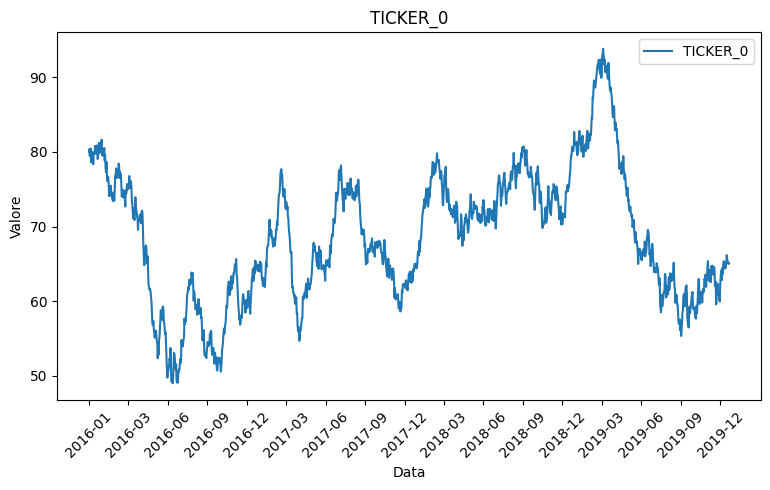
\includegraphics[width=\textwidth]{images/graficoAsset.png}
        \caption{Andamento temporale di un asset.}
        \label{fig:graficiAssets}
    \end{subfigure}
    \hfill
    \begin{subfigure}{0.45\textwidth}
        \centering
        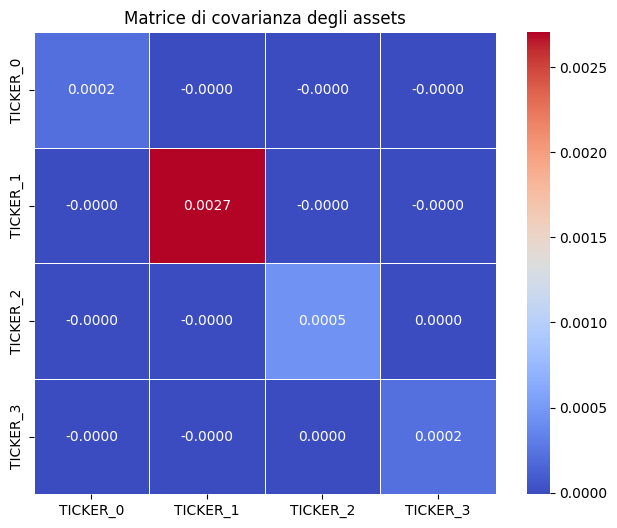
\includegraphics[width=\textwidth]{images/matriceCovarianza.png}
        \caption{Esempio di matrice di covarianza.}
        \label{fig:matriceCovarianza}
    \end{subfigure}
    \caption{Visualizzazione (a) dell'andamento dei prezzi degli asset generati, e (b) della matrice di covarianza calcolata.}
    %\label{fig:}
\end{figure}

Dopo aver calcolato i rendimenti medi e la matrice di covarianza per ciascun 
asset, procediamo con la configurazione del problema di ottimizzazione. 
Il fattore di rischio viene impostato a \textit{0.2}, permettendo di bilanciare il 
trade-off tra rendimento e rischio del portafoglio. Il budget viene definito come 
i due terzi del numero totale di asset (\texttt{assets / 3 * 2}). Viene inoltre 
definita la penalità (\texttt{penalty}) uguale al valore del budget per gestire la 
violazione dei vincoli.

Il problema viene quindi configurato attraverso l'inizializzazione di 
un'istanza della classe \texttt{PortfolioOptimization}, alla quale vengono 
passati i parametri fondamentali: il vettore dei rendimenti attesi 
(\texttt{expected\_returns}), la matrice di covarianza (\texttt{covariances}), 
il fattore di rischio e il budget. La configurazione finale produce 
un output che specifica il numero totale di asset disponibili, 
il budget allocato, la penalità impostata e il fattore di rischio 
utilizzato. Il problema viene infine convertito in un programma 
quadratico attraverso il metodo \texttt{to\_quadratic\_program} per la 
successiva ottimizzazione.

\begin{lstlisting}[language=python, caption={Configurazione del problema di ottimizzazione del portafoglio.}]
 risk_factor = 0.2
 budget = int(assets / 3 * 2)
 penalty = budget

 po = PortfolioOptimization(
     expected_returns=mu, 
     covariances=sigma, 
     risk_factor=risk_factor, 
     budget=budget
 )
 qp = po.to_quadratic_program()
\end{lstlisting}

\paragraph{Risoluzione classica del problema}
Per ottenere una soluzione di riferimento al nostro problema di ottimizzazione, 
utilizziamo un approccio classico basato su autovalori. In particolare, 
impieghiamo il risolutore \texttt{NumPyMinimumEigensolver}, un algoritmo 
che calcola in modo esatto gli autovalori del problema. Questo risolutore 
viene integrato attraverso \texttt{MinimumEigenOptimizer}, un wrapper  
che fornisce un'interfaccia conveniente per utilizzare il solver e
risolvere il problema di ottimizzazione.

\begin{lstlisting}[language=python, caption={Risoluzione classica del problema utilizzando \texttt{NumPyMinimumEigensolver.}}]
 exact_mes = NumPyMinimumEigensolver()
 exact_eigensolver = MinimumEigenOptimizer(exact_mes)
 result = exact_eigensolver.solve(qp)
\end{lstlisting}

Questa implementazione classica serve come benchmark fondamentale per 
valutare le prestazioni dei metodi quantistici che verranno 
implementati successivamente.

Si può osservare che nel risultato ottenuto nella Figura~\ref{fig:risultatoClassico}, il risolutore 
classico fornisce un unico risultato, il quale corrisponde a quello ottimale, con una probabilità 
del 100\%. Come già discusso nella Sezione~\ref{sec:problema}, questo metodo 
è rapido quando tratta un numero ridotto di asset, ma diventa sempre più lento 
man mano che il numero di quest'ultimi aumenta. In definitiva, come già accennato, 
l'obiettivo principale del quantum computing non è tanto migliorare il 
risultato ottenuto, quanto piuttosto accelerare la risoluzione dei problemi.

\paragraph{Risoluzione con VQE}
\paragraph{Risoluzione con QAOA}




\begin{figure}[h!]
    \centering
    \begin{subfigure}{0.49\textwidth}
        \centering
        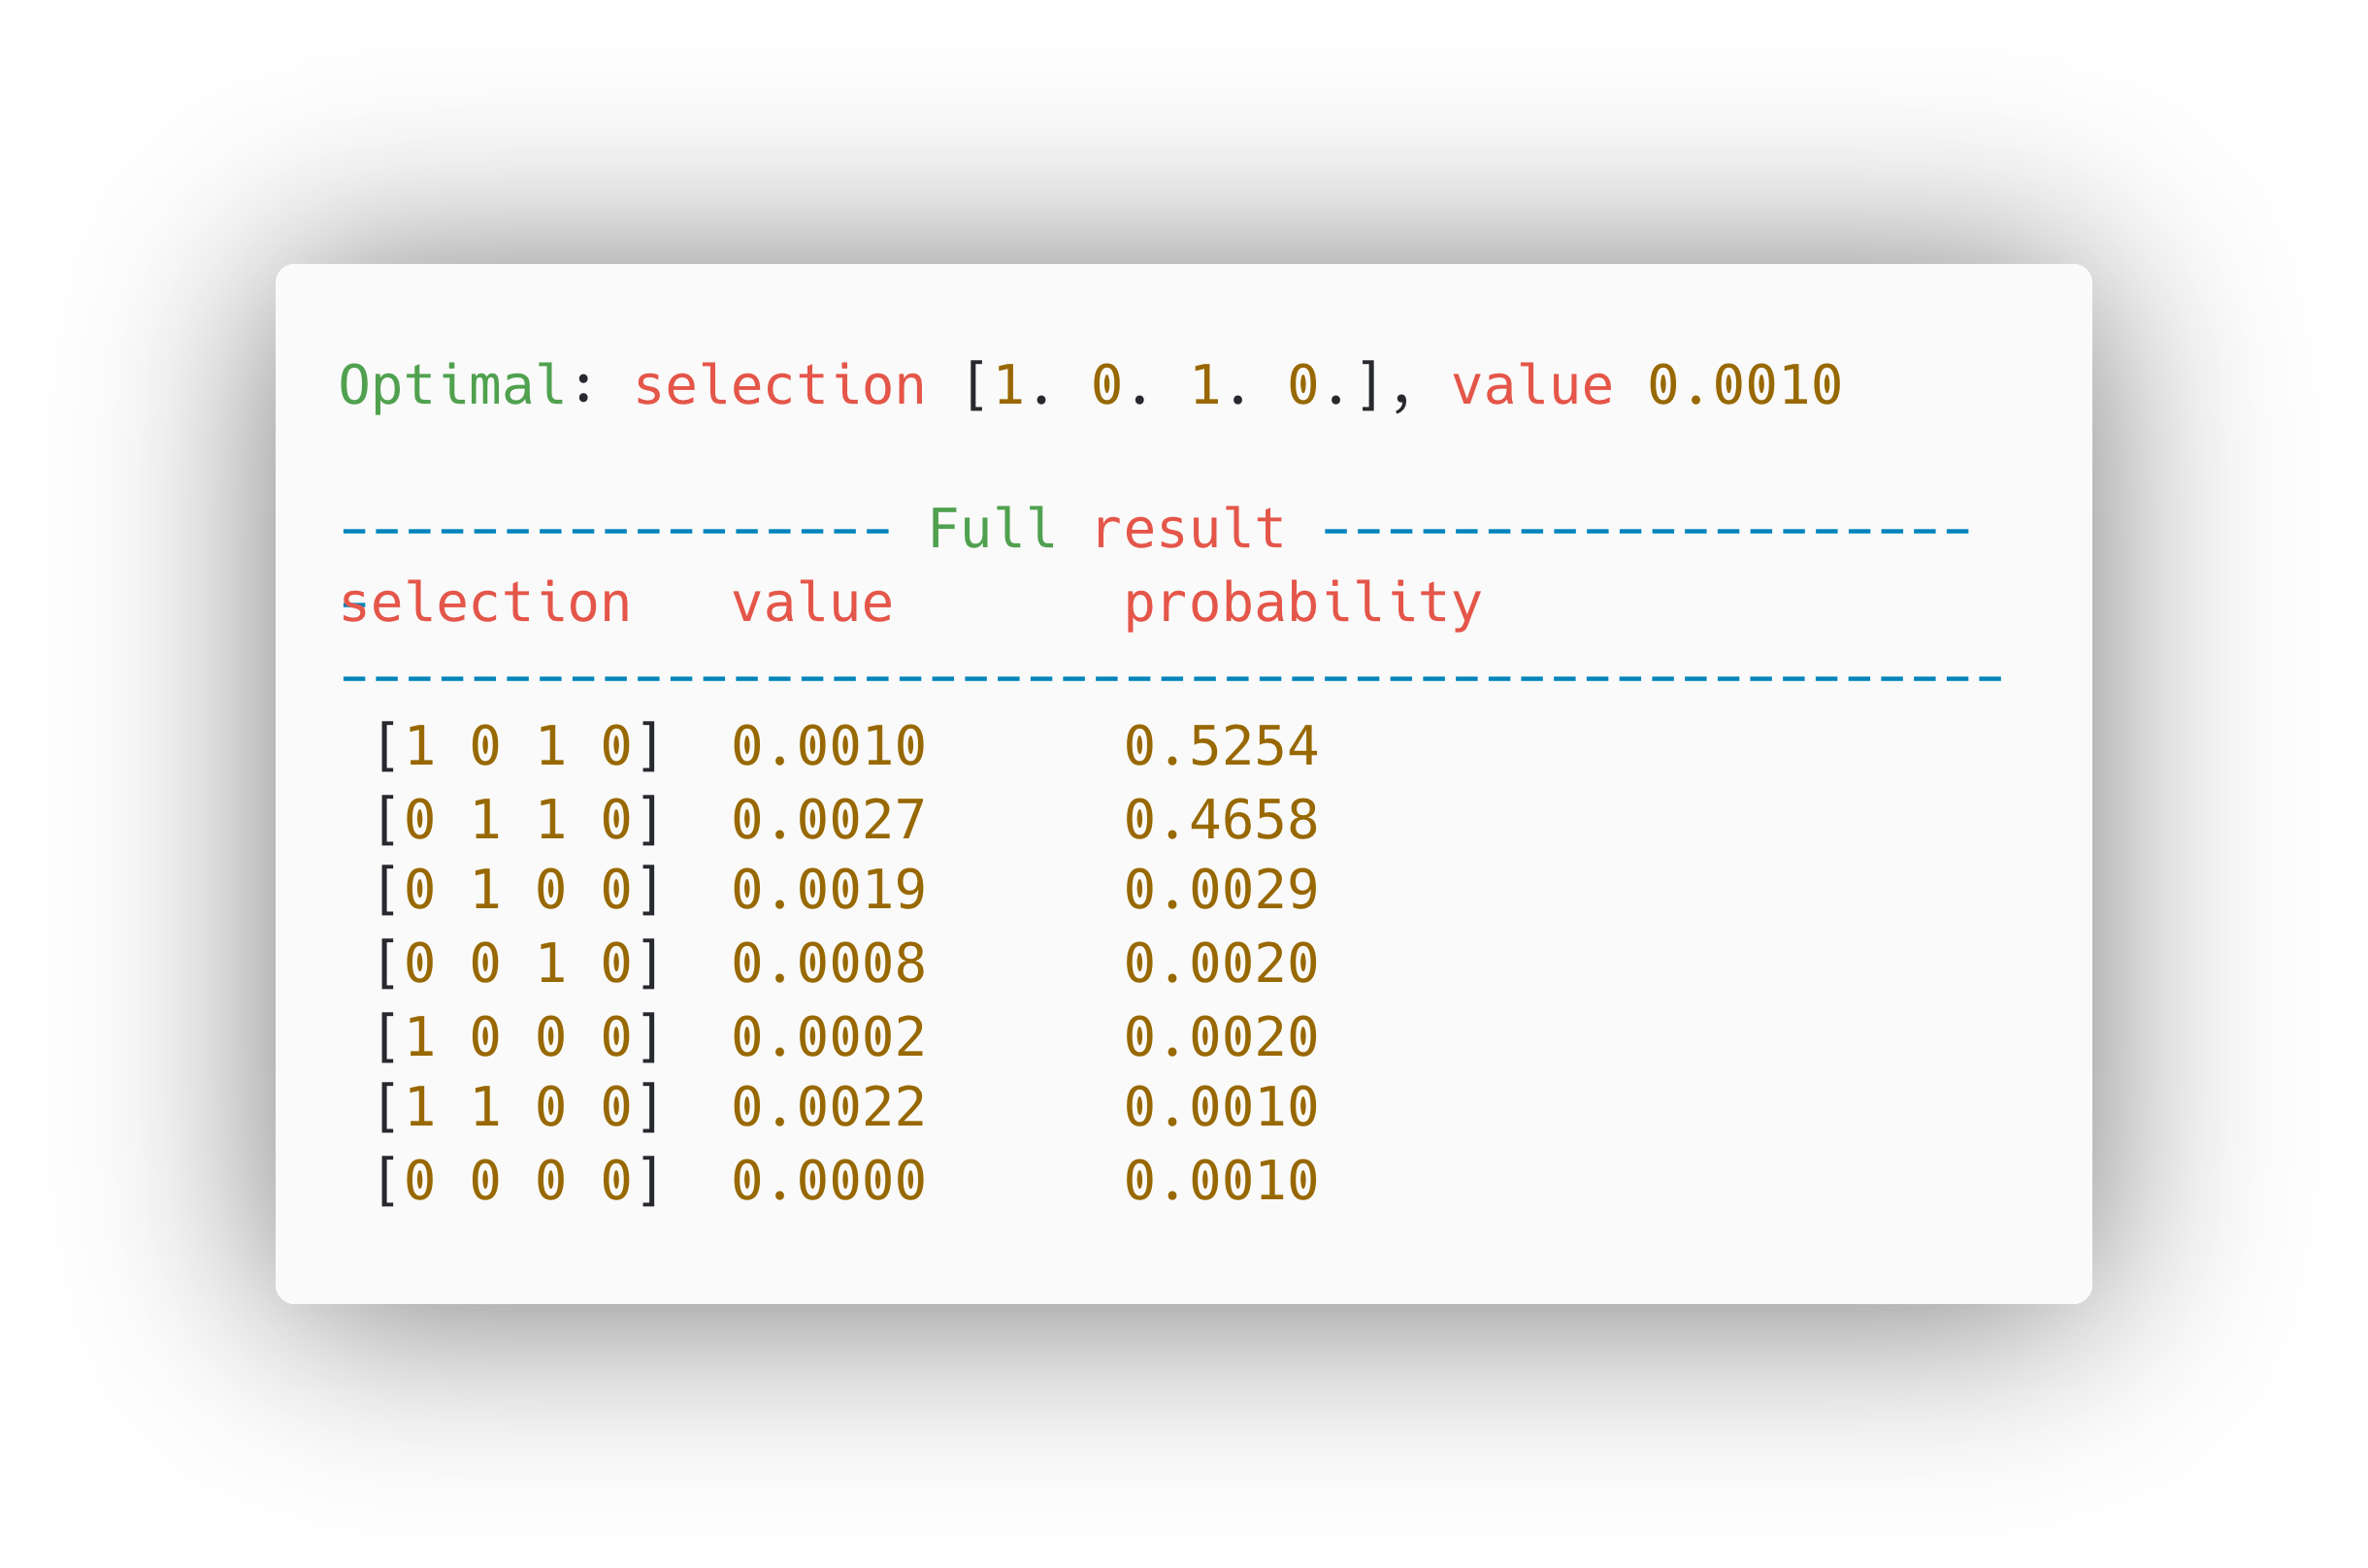
\includegraphics[width=\textwidth]{images/risultatoVQE.png}
        \caption{Risultato ottenuto con VQE.}
        \label{fig:risultatoVQE}
    \end{subfigure}
    \hfill
    \begin{subfigure}{0.49\textwidth}
        \centering
        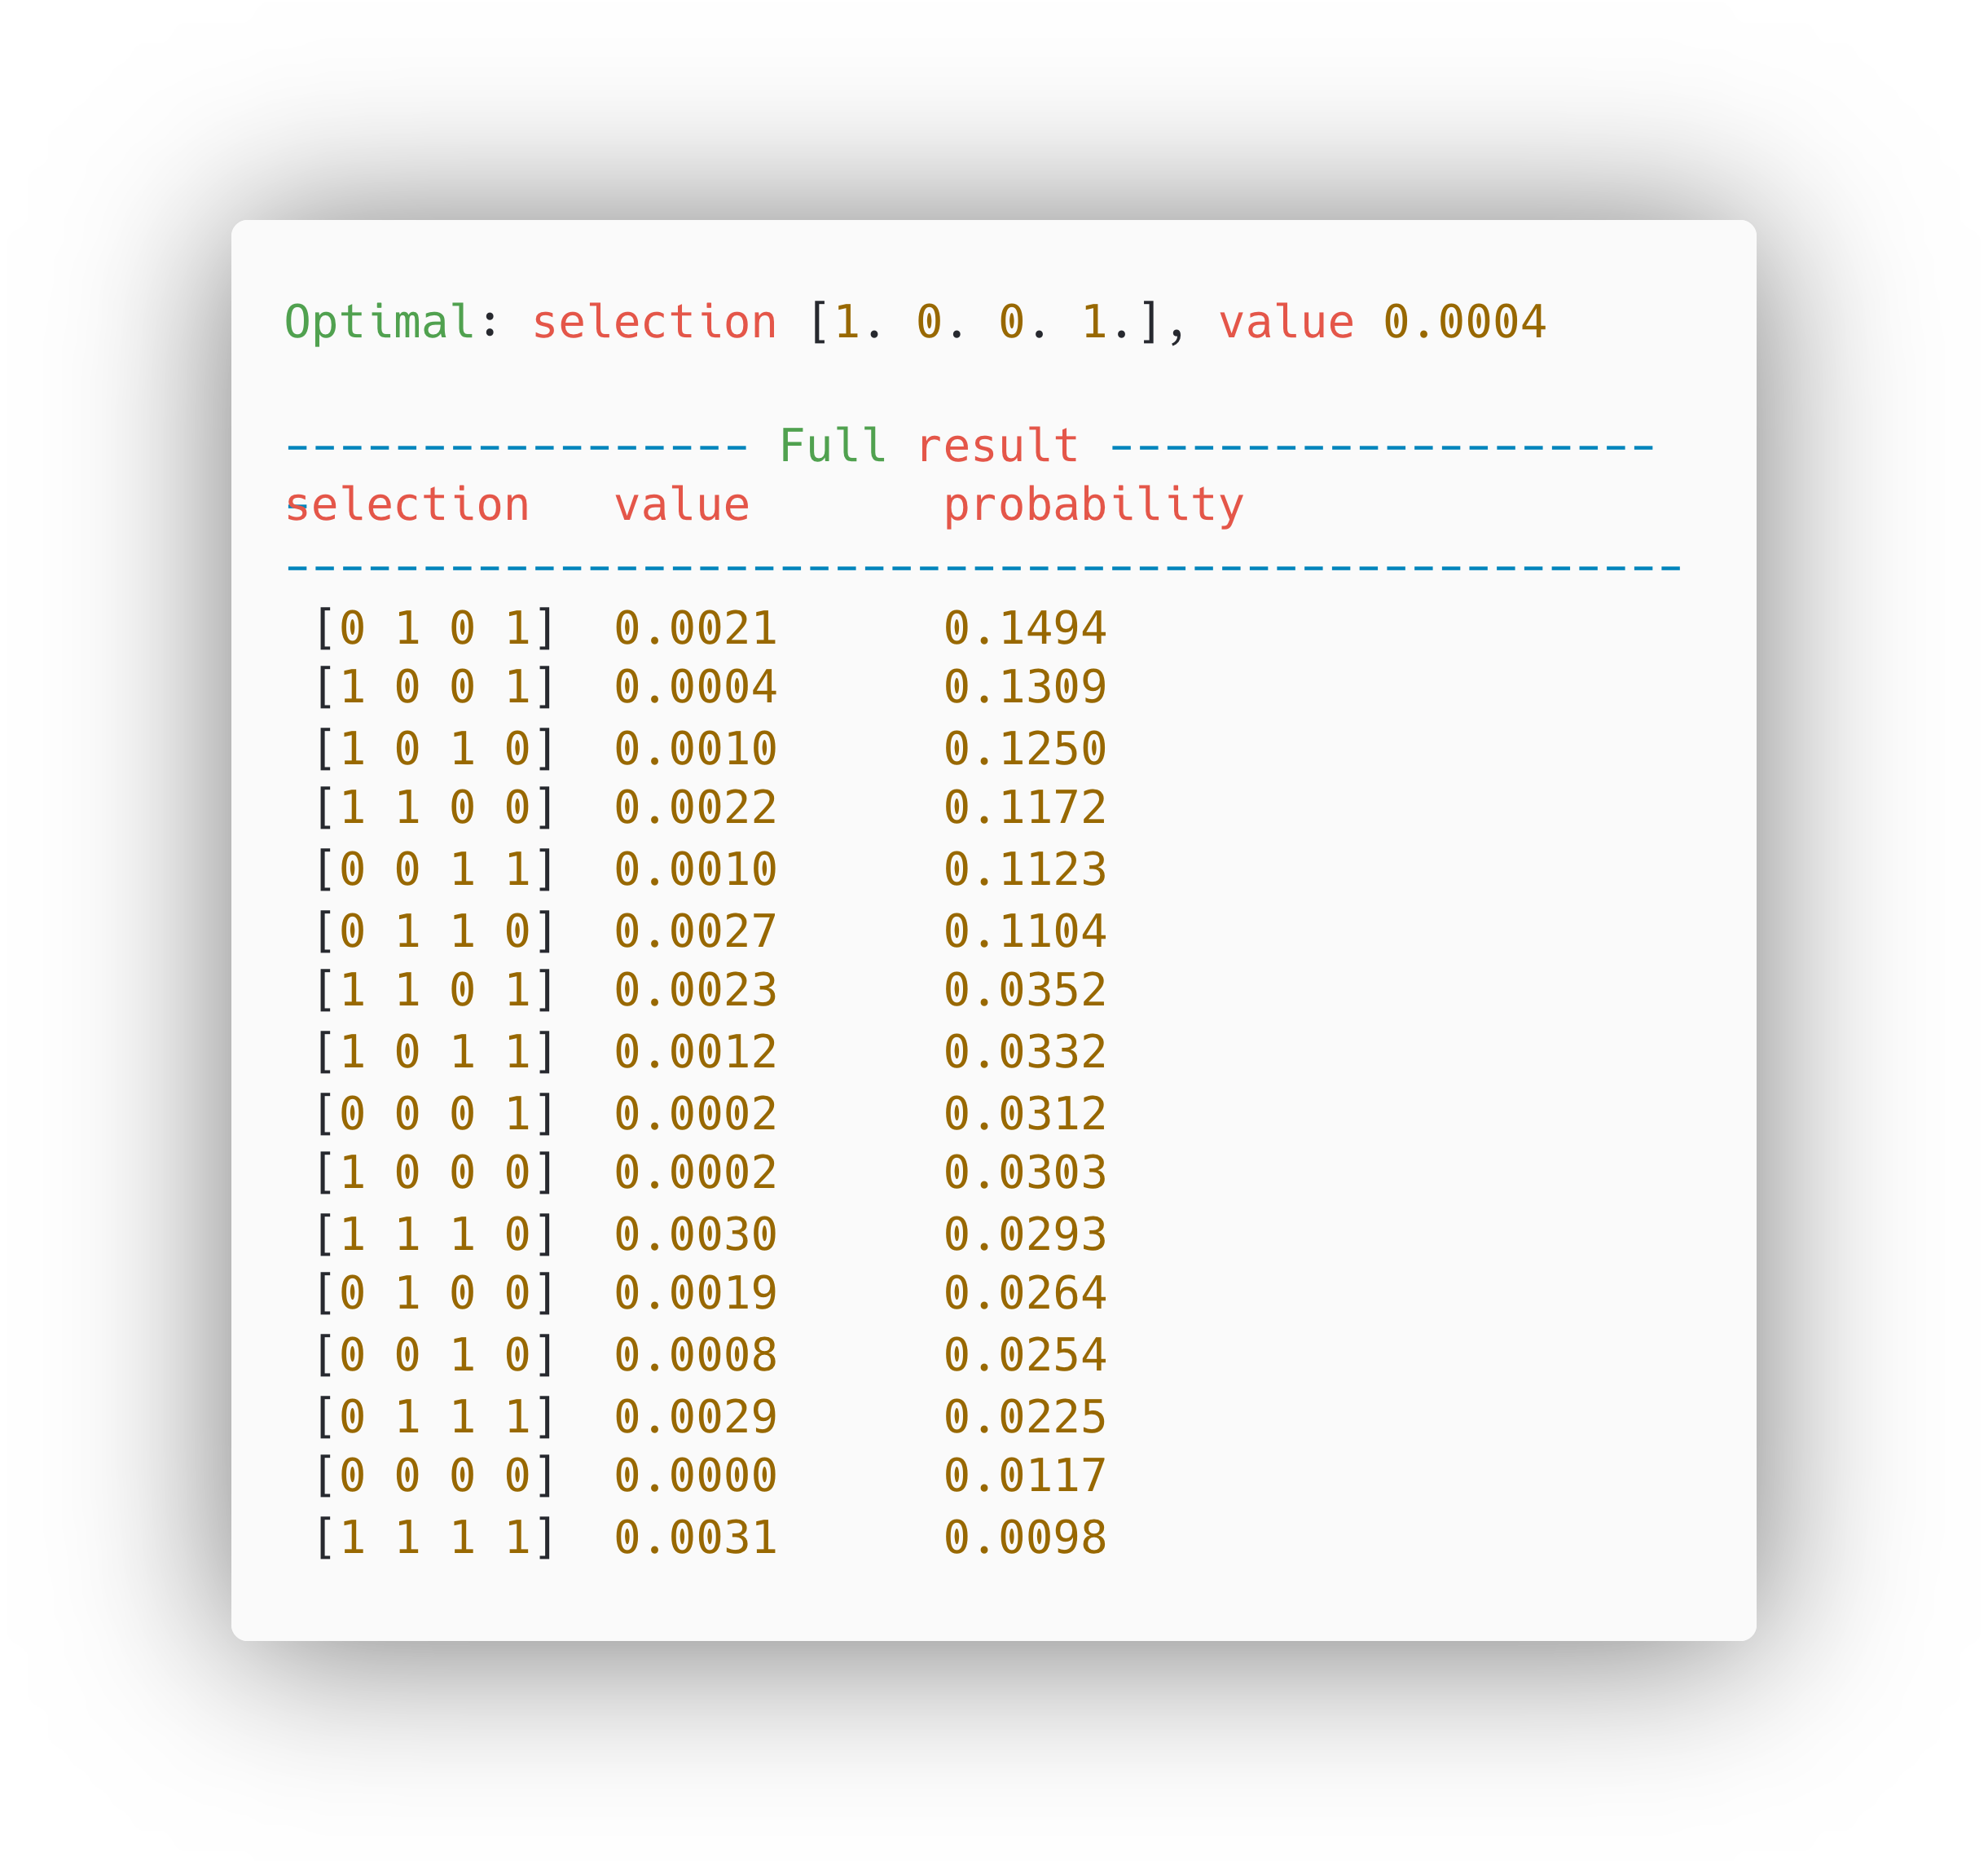
\includegraphics[width=\textwidth]{images/risultatoQAOA.png}
        \caption{Risultato ottenuto con QAOA.}
        \label{fig:risultatoQAOA}
    \end{subfigure}
    \hfill
    \begin{subfigure}{0.60\textwidth}
        \centering
        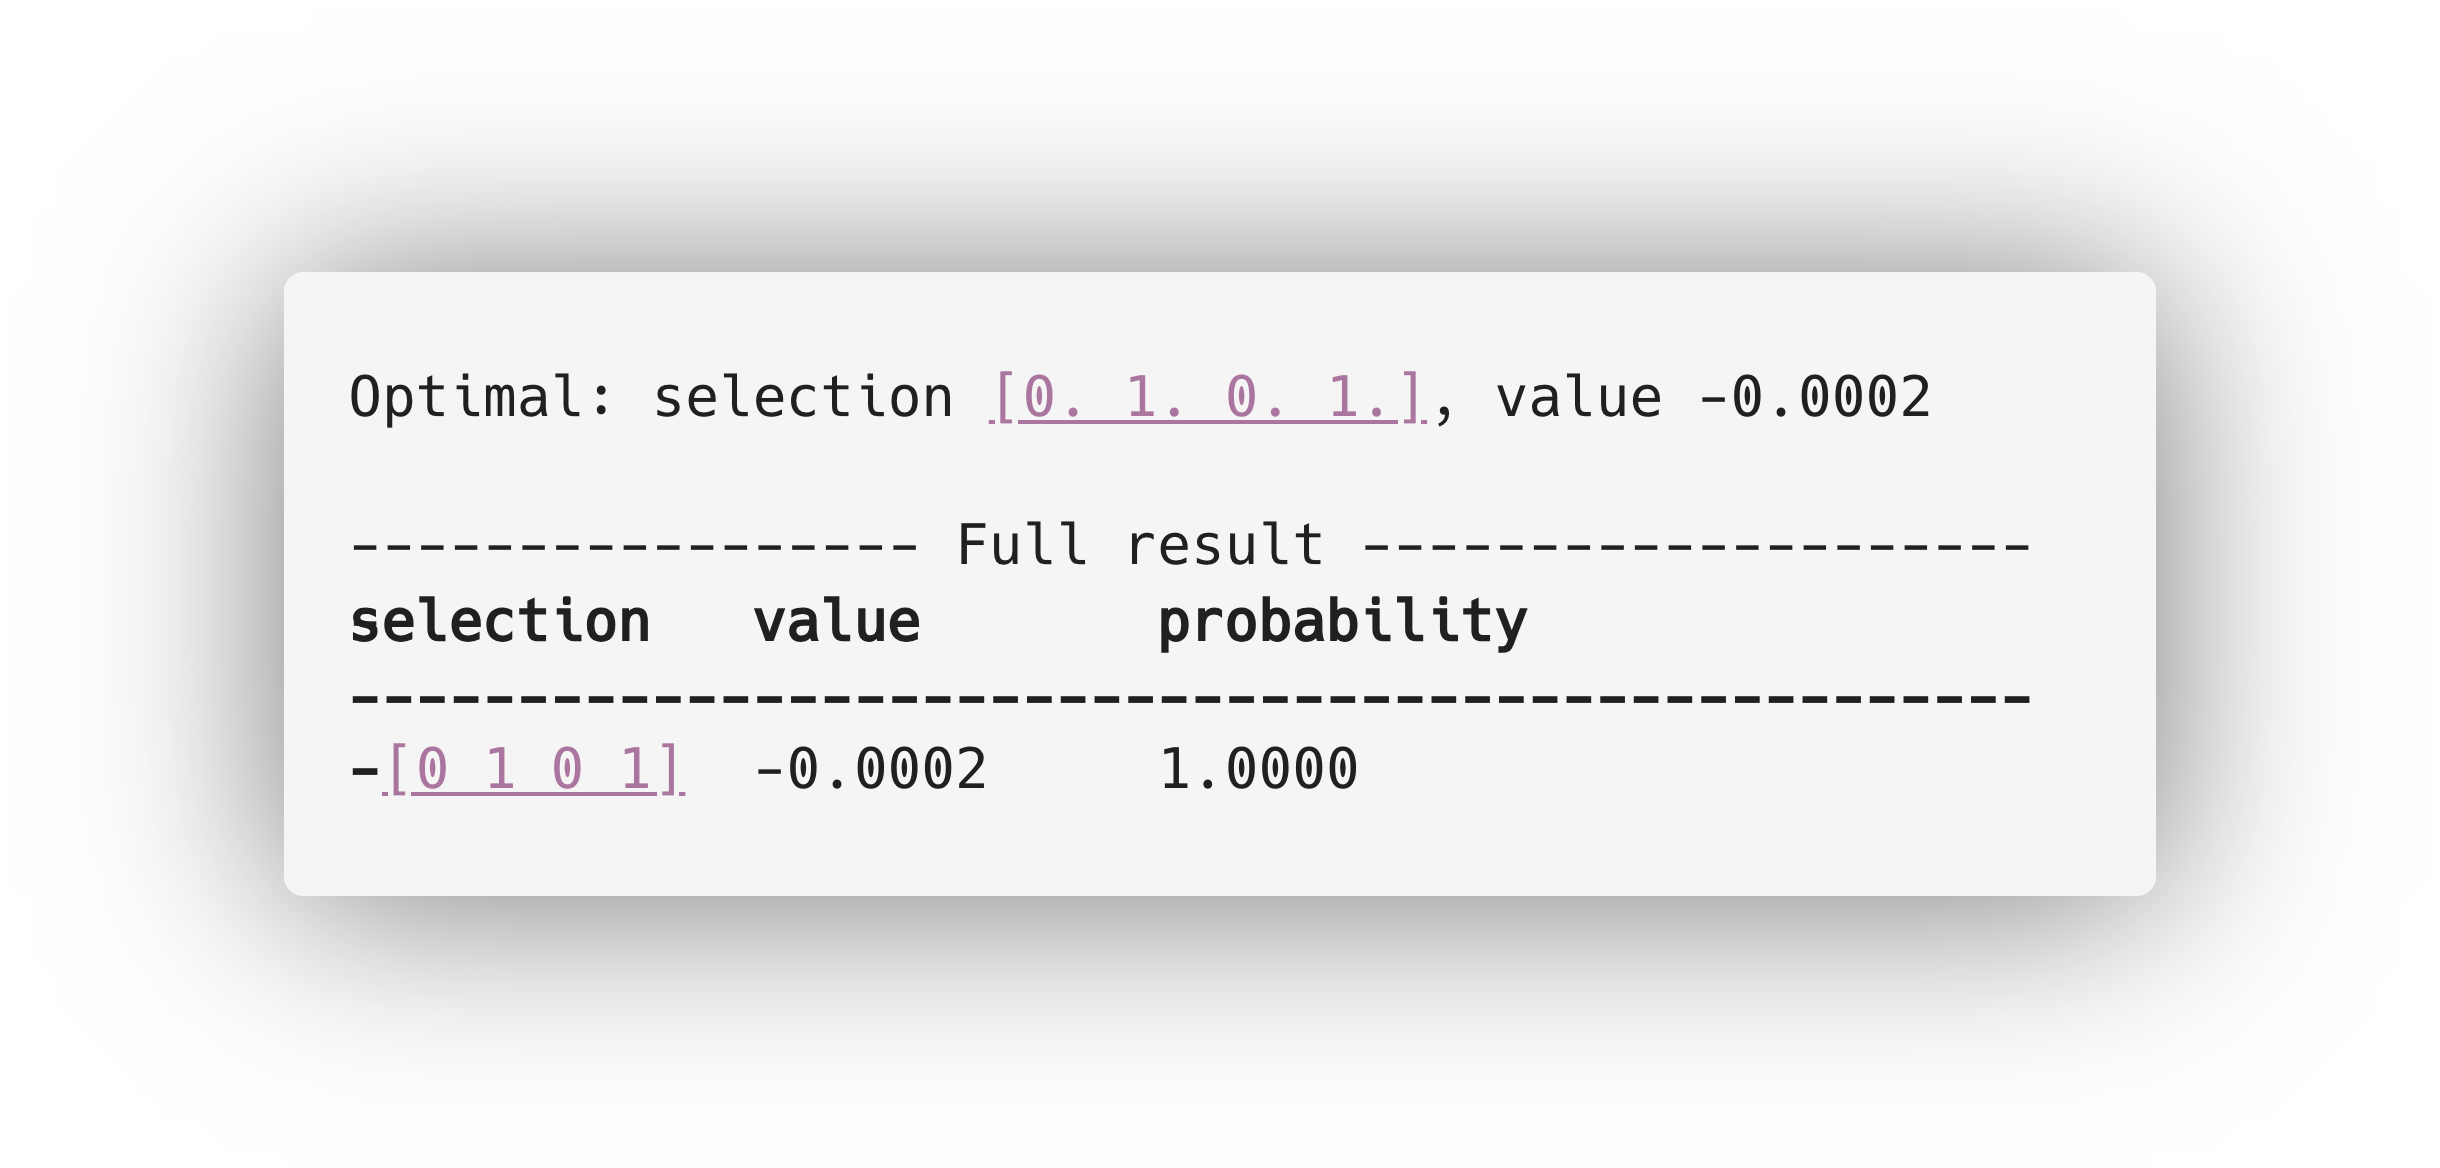
\includegraphics[width=\textwidth]{images/risultatoClassico.png}
        \caption{Risultato ottenuto con il risolutore classico.}
        \label{fig:risultatoClassico}
    \end{subfigure}
    \caption{Risultati ottenuti con (a) VQE, (b) QAOA e (c) risolutore classico.}
    %\label{fig:}
\end{figure}